\documentclass[5pt]{article}
    \title{\textbf{1. MĚŘENÍ ANALOGOVÝM OSCILOSKOPEM}}
    \author{Tomáš Kysela}
    \date{16/2/2022}
    
    \addtolength{\topmargin}{-3cm}
    \addtolength{\textheight}{3cm}
    
\usepackage[czech]{babel}
\usepackage{graphicx}
\usepackage{circuitikz}
\usepackage{amsmath}
\usepackage{subcaption}
\begin{document}

\maketitle
\thispagestyle{empty}

\section{Úkol měření}
\begin{enumerate}
\item Na základě popisu uvedeného v Teoretickém úvodu se  seznamte  s funkcí analogového laboratorního osciloskopu.
\item S použitím jednokanálového režimu zobrazte na analogovém osciloskopu průběh napětí v bodě K1 popř. K2  astabilního  klopného  obvodu.  Zesílení,  vertikální  posuv (skupina  ovládacích  prvků „vertical“)  a rychlost běhu ČZ (skupina ovládacích prvků „horizontal“) nastavte tak, aby zobrazení bylo optimální. Nastavte režim spouštění „AUTO“ signálem z použitého kanálu, sledujte vliv změny nastavení  spouštěcí  úrovně,  popř.  spouštění  náběžnou  a  sestupnou  hranou  na  zobrazený  signál (skupina ovládacích prvků „trigger“). Totéž vyzkoušejte v režimu „NORM“.
\item U zobrazeného průběhu určete frekvenci, $U_{min}$,  $U_{max}$, střední hodnotu (stejnosměrnou složku), trvání vzestupné  a  sestupné  hrany.  Pozor,  hodnoty  pro  rychlost  běhu  ČZ  a  citlivosti  platí  pouze  jsou-li plynulá nastavení v poloze „kalibrováno“ (cal).
\item S použitím dvoukanálového režimu zobrazte na analogovém osciloskopu průběhy  napětí v bodě K1 popř. K2 a B1 popř. B2 astabilního klopného obvodu.
\item S využitím nf generátoru a napětí 6 V o kmitočtu 50 Hz (z rozvaděče) ověřte funkci režimu X-Y osciloskopu (Lissajoussovy obrazce).
\item Body  2  a  3  zopakujte  s použitím číslicového osciloskopu (popis ovládacích prvků je podobný). Pro základní nastavení ovládacích prvků použijte tlačítko „Auto Scale“. Povšimněte si rozdílů v zobrazení (bod  „trig“  je  při  základním  nastavení  uprostřed  a  je  tedy  zobrazen  i  průběh  signálu  před  jeho průchodem spouštěcí úrovní). Pro měření parametrů vstupního signálu kromě odečtení ze zobrazeného průběhu,  jako  tomu  bylo  v případě  analogového  osciloskopu,  použijte  i  režim  „Measure“,  pokud změření těchto parametrů umožňuje. Výsledky porovnejte.
\end{enumerate}
\newpage

\section{Schéma zapojení­}
\begin{figure}[htp]
\centering
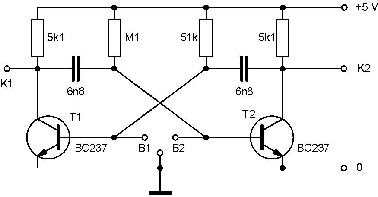
\includegraphics[scale=1.00]{scheme.png}
\caption{Schéma zapojení astabilního klopného obvodu s vyznačenými měřicími body}
\end{figure}
\begin{figure}[htp]
\centering
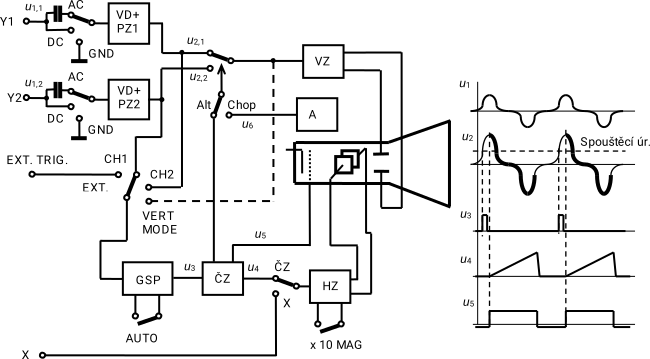
\includegraphics[scale=0.8]{block.png}
\caption{Osciloskop}
\end{figure}

\section{Soupis použitých přístrojů}

\begin{tabular}{ll}
	Analogový osciloskop & GOLDSTAR OS-904RD\\
	Číslicový osciloskop\\
	Generátor funkcí
\end{tabular}

\section{Teoretický úvod}
Obvyklý režim činnosti osciloskopu zobrazuje časový průběh signálů. Existuje však i tzv. režim X-Y, kdz je napětí přivedené na vstup osciloskopu zobrazeno jako funkce napětí přivedeného na horizontální vstup.
Osciloskop má dva základní vstupy - vertikální vstup Y a horizontální X.\\
V případě standartního režimu je použit pouze kanál Y. Přepínač následně umožňuje následující funkce\\
AC) Připojí mezi vstup oscilátoru a vstupní dělič kondenzátor a tím odfiltruje stejnosměrnou složku.\\
GND) Uzemní vstup oscilátoru a tím umožňuje nastavení nuly.\\
DC) Přivádí vstup přímo na vstupní dělič a tak ukazuje neměný signál.\\
Pro zobrazení časového průběh vstupního napětí na stínítku obrazovky je nutné, aby se současně svítící bod pohyboval rovnoměrně zleva doprava. Rovnoměrný horizontální posuv svítícího bodu od levého okraje stínítka k pravému zajišťuje pilové napětí u4 generované obvodem nazývaným časová základna ČZ, zesilované horizontálním zesilovačem HZ a přivedené na horizontálně vychylující destičky. Zesílení HZ lze zvětšit 10 x pomocí ovládacího prvku „x10 MAG“ a tak dosáhnout desetinásobného
roztažení zobrazení

\section{Tabulky hodnot}
\subsection{Úkol 3}
\begin{tabular}{r|l}
	$ \Delta T $ & $ 0.172 ms $\\ \hline \\
	$ f $ & $ 1.404 kHz $\\ \hline \\
	$ U_{min} $ & $ 0 V $\\ \hline \\
	$ U_{min} $ & $ 4.32 V $\\ \hline \\
	$ U_{sa} $ & $ -1.32 V $\\ \hline \\
	$ t_n $ & $ 83.6 \mu s $ \\ \hline \\
	$ t_s $ & $ 1 \mu s $ \\
\end{tabular}

\subsection{Úkol 4}
\begin{figure}[htp]
\centering
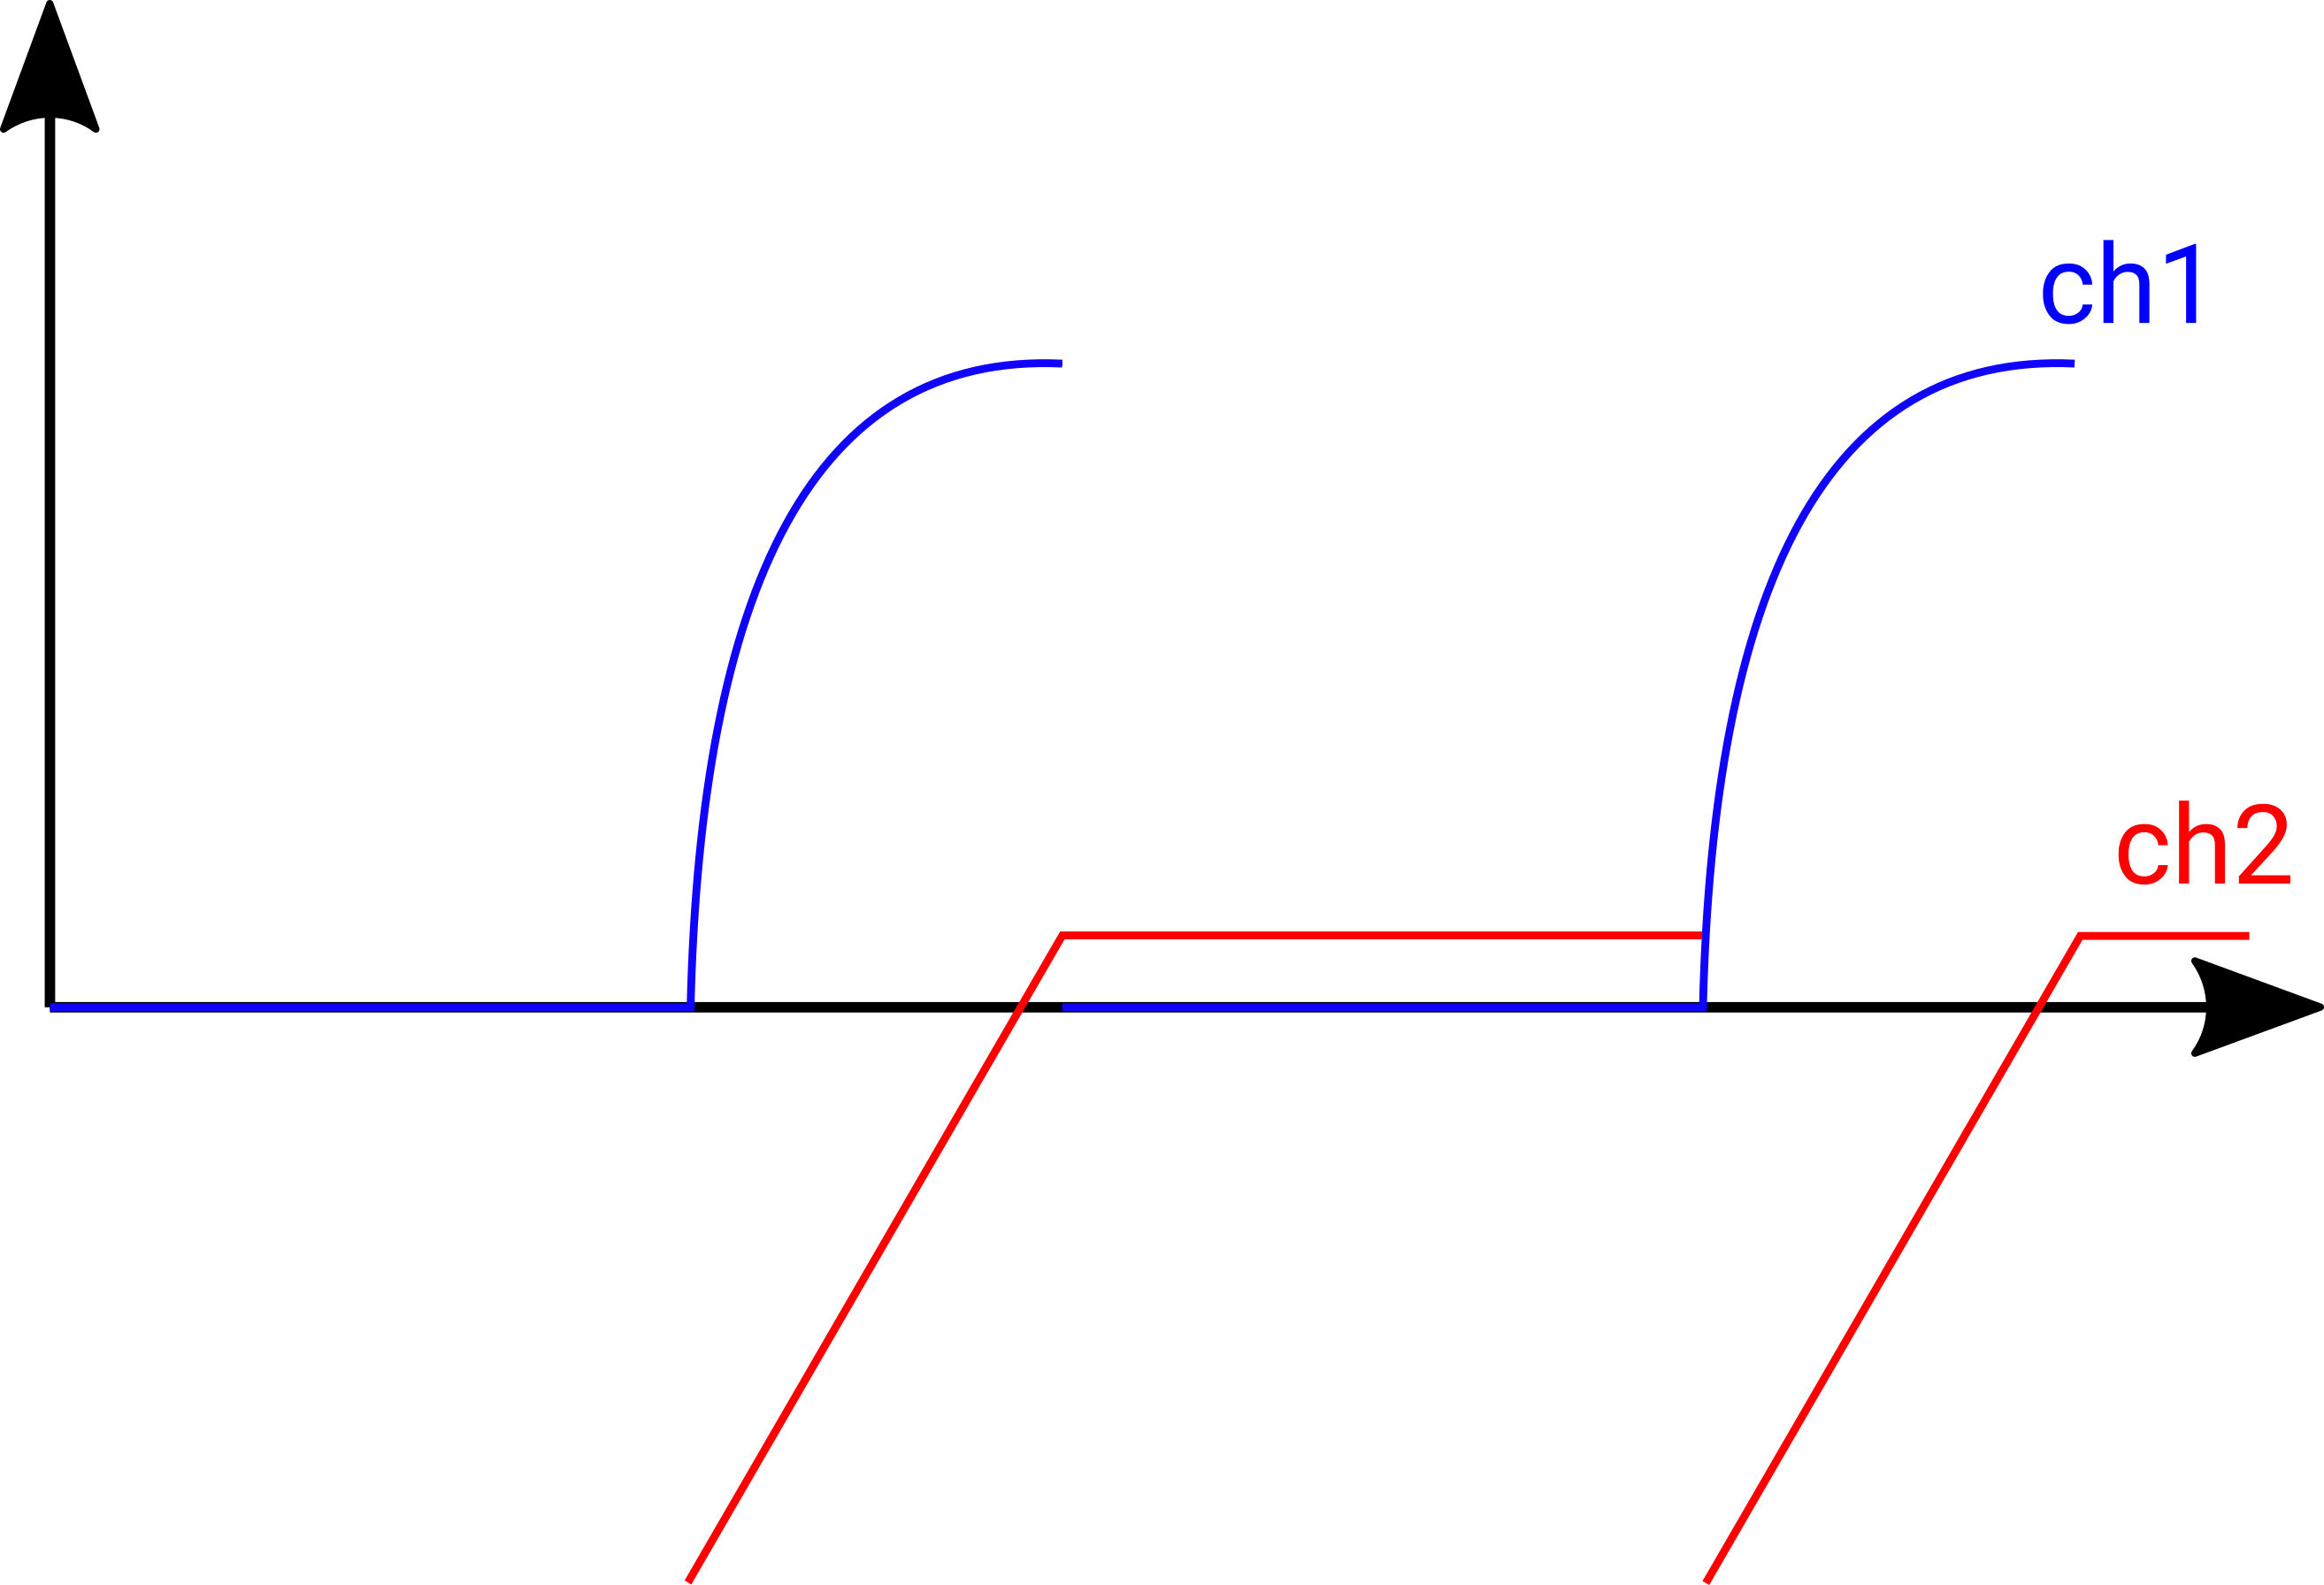
\includegraphics[scale=0.35]{graph.png}
\caption{}
\label{}
\end{figure}
\subsection{Úkol 5}
\begin{figure}[htp]
\centering
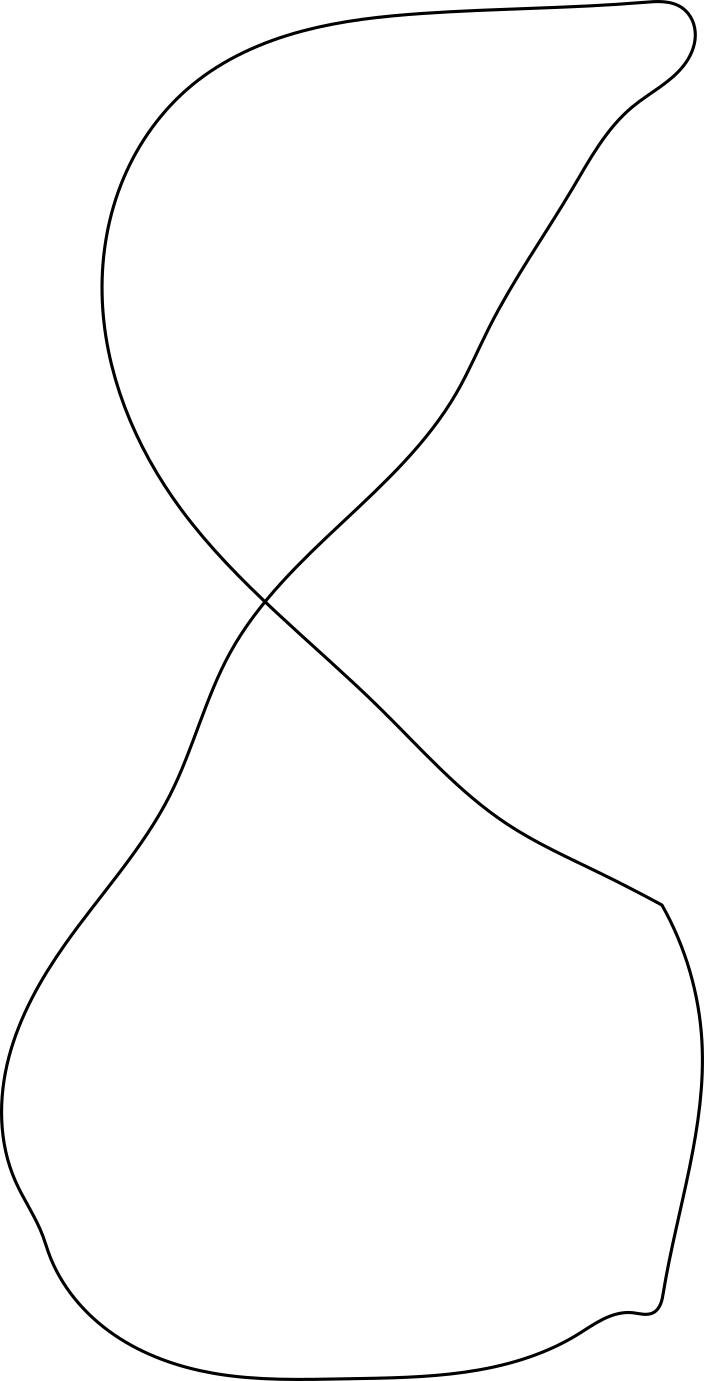
\includegraphics[scale=0.35]{graph2.png}
\caption{Rotující Lassajoussův obrazec}
\label{}
\end{figure}
\subsection{Úkol 6}
\begin{tabular}{r|l}
	$ f $ & $ 1.395 kHz $\\ \hline \\
	$ U_{min} $ & $ -1.36 V $\\ \hline \\
	$ U_{min} $ & $ 3 V $\\ \hline \\
	$ U_{sa} $ & $ -1.36 V $\\ \hline \\
	$ t_n $ & $ 80 \mu s $ \\ \hline \\
	$ t_s $ & $ 146 ns $ \\
\end{tabular}

\section{Závěr}
Meření pomocí obou metod bylo úspešné, avšak maximální a minimální hodnotu v části 3 jsem měřil v režimu AC a tedy nebyla započítáná stejnosměrná složka. Všechny ostatní hodnoty jsou s minimální odchylkou a Lassajoussovi obrazce byly úspěšně zobrazeny...
\end{document}
